% === Exercise 8.4.2 ===
\begin{Exercise}
\begin{enumerate}[a)]
\item
\begin{sketch} 
See the Figure \ref{fig:8.4.2_a}.

\begin{minipage}[h]{0.9\textwidth}
\centering
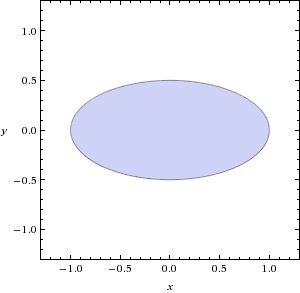
\includegraphics[width=6cm]{fig_8_4_2_a}
\captionof{figure}{}
\label{fig:8.4.2_a}
\end{minipage}

$E^\circ = \{(x,y):x^2+4y^2< 1\}$.

$\overline{\rm E} = E = \{(x,y):x^2+4y^2 \leq 1\}$.

$\partial E = \{(x,y):x^2+4y^2 = 1\}$.
\end{sketch}

\item
\begin{sketch} 
See the Figure \ref{fig:8.4.2_b}.

\begin{minipage}[h]{0.9\textwidth}
\centering
\definecolor{ffqqqq}{rgb}{1.,0.,0.}
\begin{tikzpicture}[line cap=round,line join=round,>=triangle 45,x=1.0cm,y=1.0cm]
\draw[->,color=black] (-1.,0.) -- (4.,0.);
\foreach \x in {-1.,1.,2.,3.}
\draw[shift={(\x,0)},color=black] (0pt,2pt) -- (0pt,-2pt) node[below] {\footnotesize $\x$};
\draw[->,color=black] (0.,-2.) -- (0.,2.);
\foreach \y in {-2.,-1.,1.}
\draw[shift={(0,\y)},color=black] (2pt,0pt) -- (-2pt,0pt) node[left] {\footnotesize $\y$};
\draw[color=black] (0pt,-10pt) node[right] {\footnotesize $0$};
\clip(-1.,-2.) rectangle (4.,2.);
\draw [line width=2.pt,color=ffqqqq] (1.,0.) circle (1.cm);
\draw [line width=2.pt,color=ffqqqq] (2.,0.)-- (3.,0.);
\end{tikzpicture}
\captionof{figure}{}
\label{fig:8.4.2_b}
\end{minipage}

$E^\circ = \phi$.

$\overline{\rm E} = E = \{(x,y):x^2-2x+y^2=0\}\cup\{(x,0):x\in[2,3]\}$.

$\partial E = E = \{(x,y):x^2-2x+y^2=0\}\cup\{(x,0):x\in[2,3]\}$.
\end{sketch}

\item
\begin{sketch} 
See the Figure \ref{fig:8.4.2_c}.

\begin{minipage}[h]{0.9\textwidth}
\centering
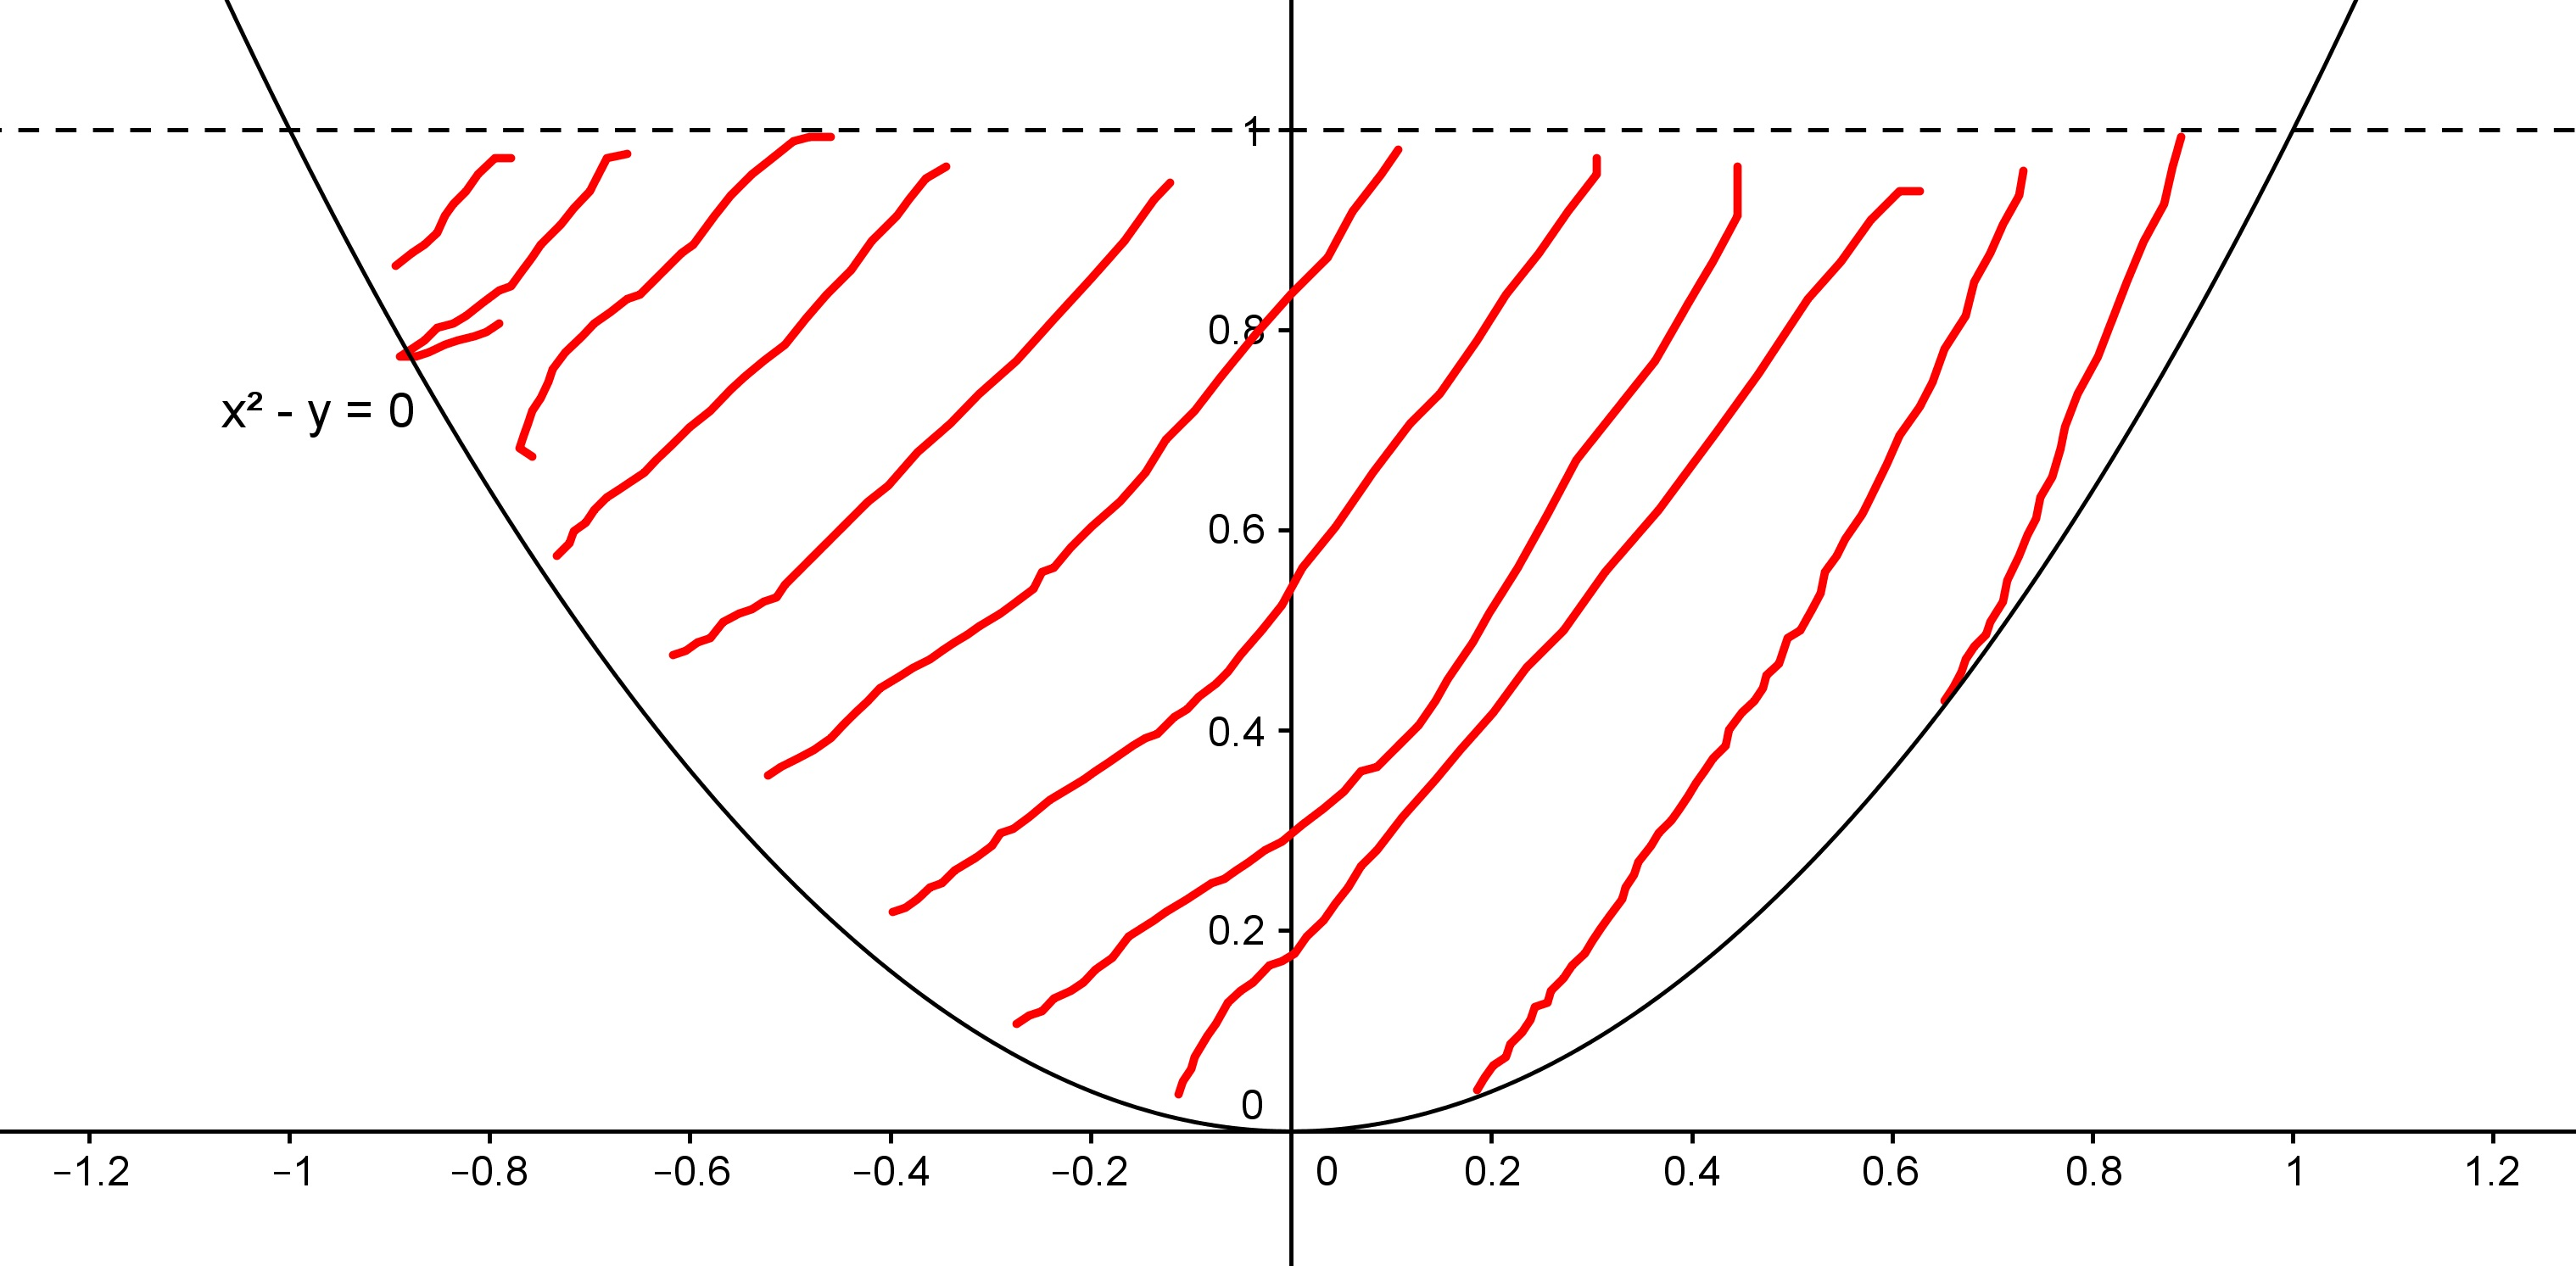
\includegraphics[width=0.7\textwidth]{fig_8_4_2_c}
\captionof{figure}{}
\label{fig:8.4.2_c}
\end{minipage}

$E^\circ = \{(x,y):y>x^2,0<y<1\}$.

$\overline{\rm E} = \{(x,y):y\geq x^2, 0\leq y \leq 1\}$.

$\partial E = \{(x,y):y=x^2,0\leq y \leq 1\}\cup\{(x,1):-1\leq x\leq 1\}$.
\end{sketch}

\item
\begin{sketch} 
See the Figure \ref{fig:8.4.2_d}.

\begin{minipage}[h]{0.9\textwidth}
\centering
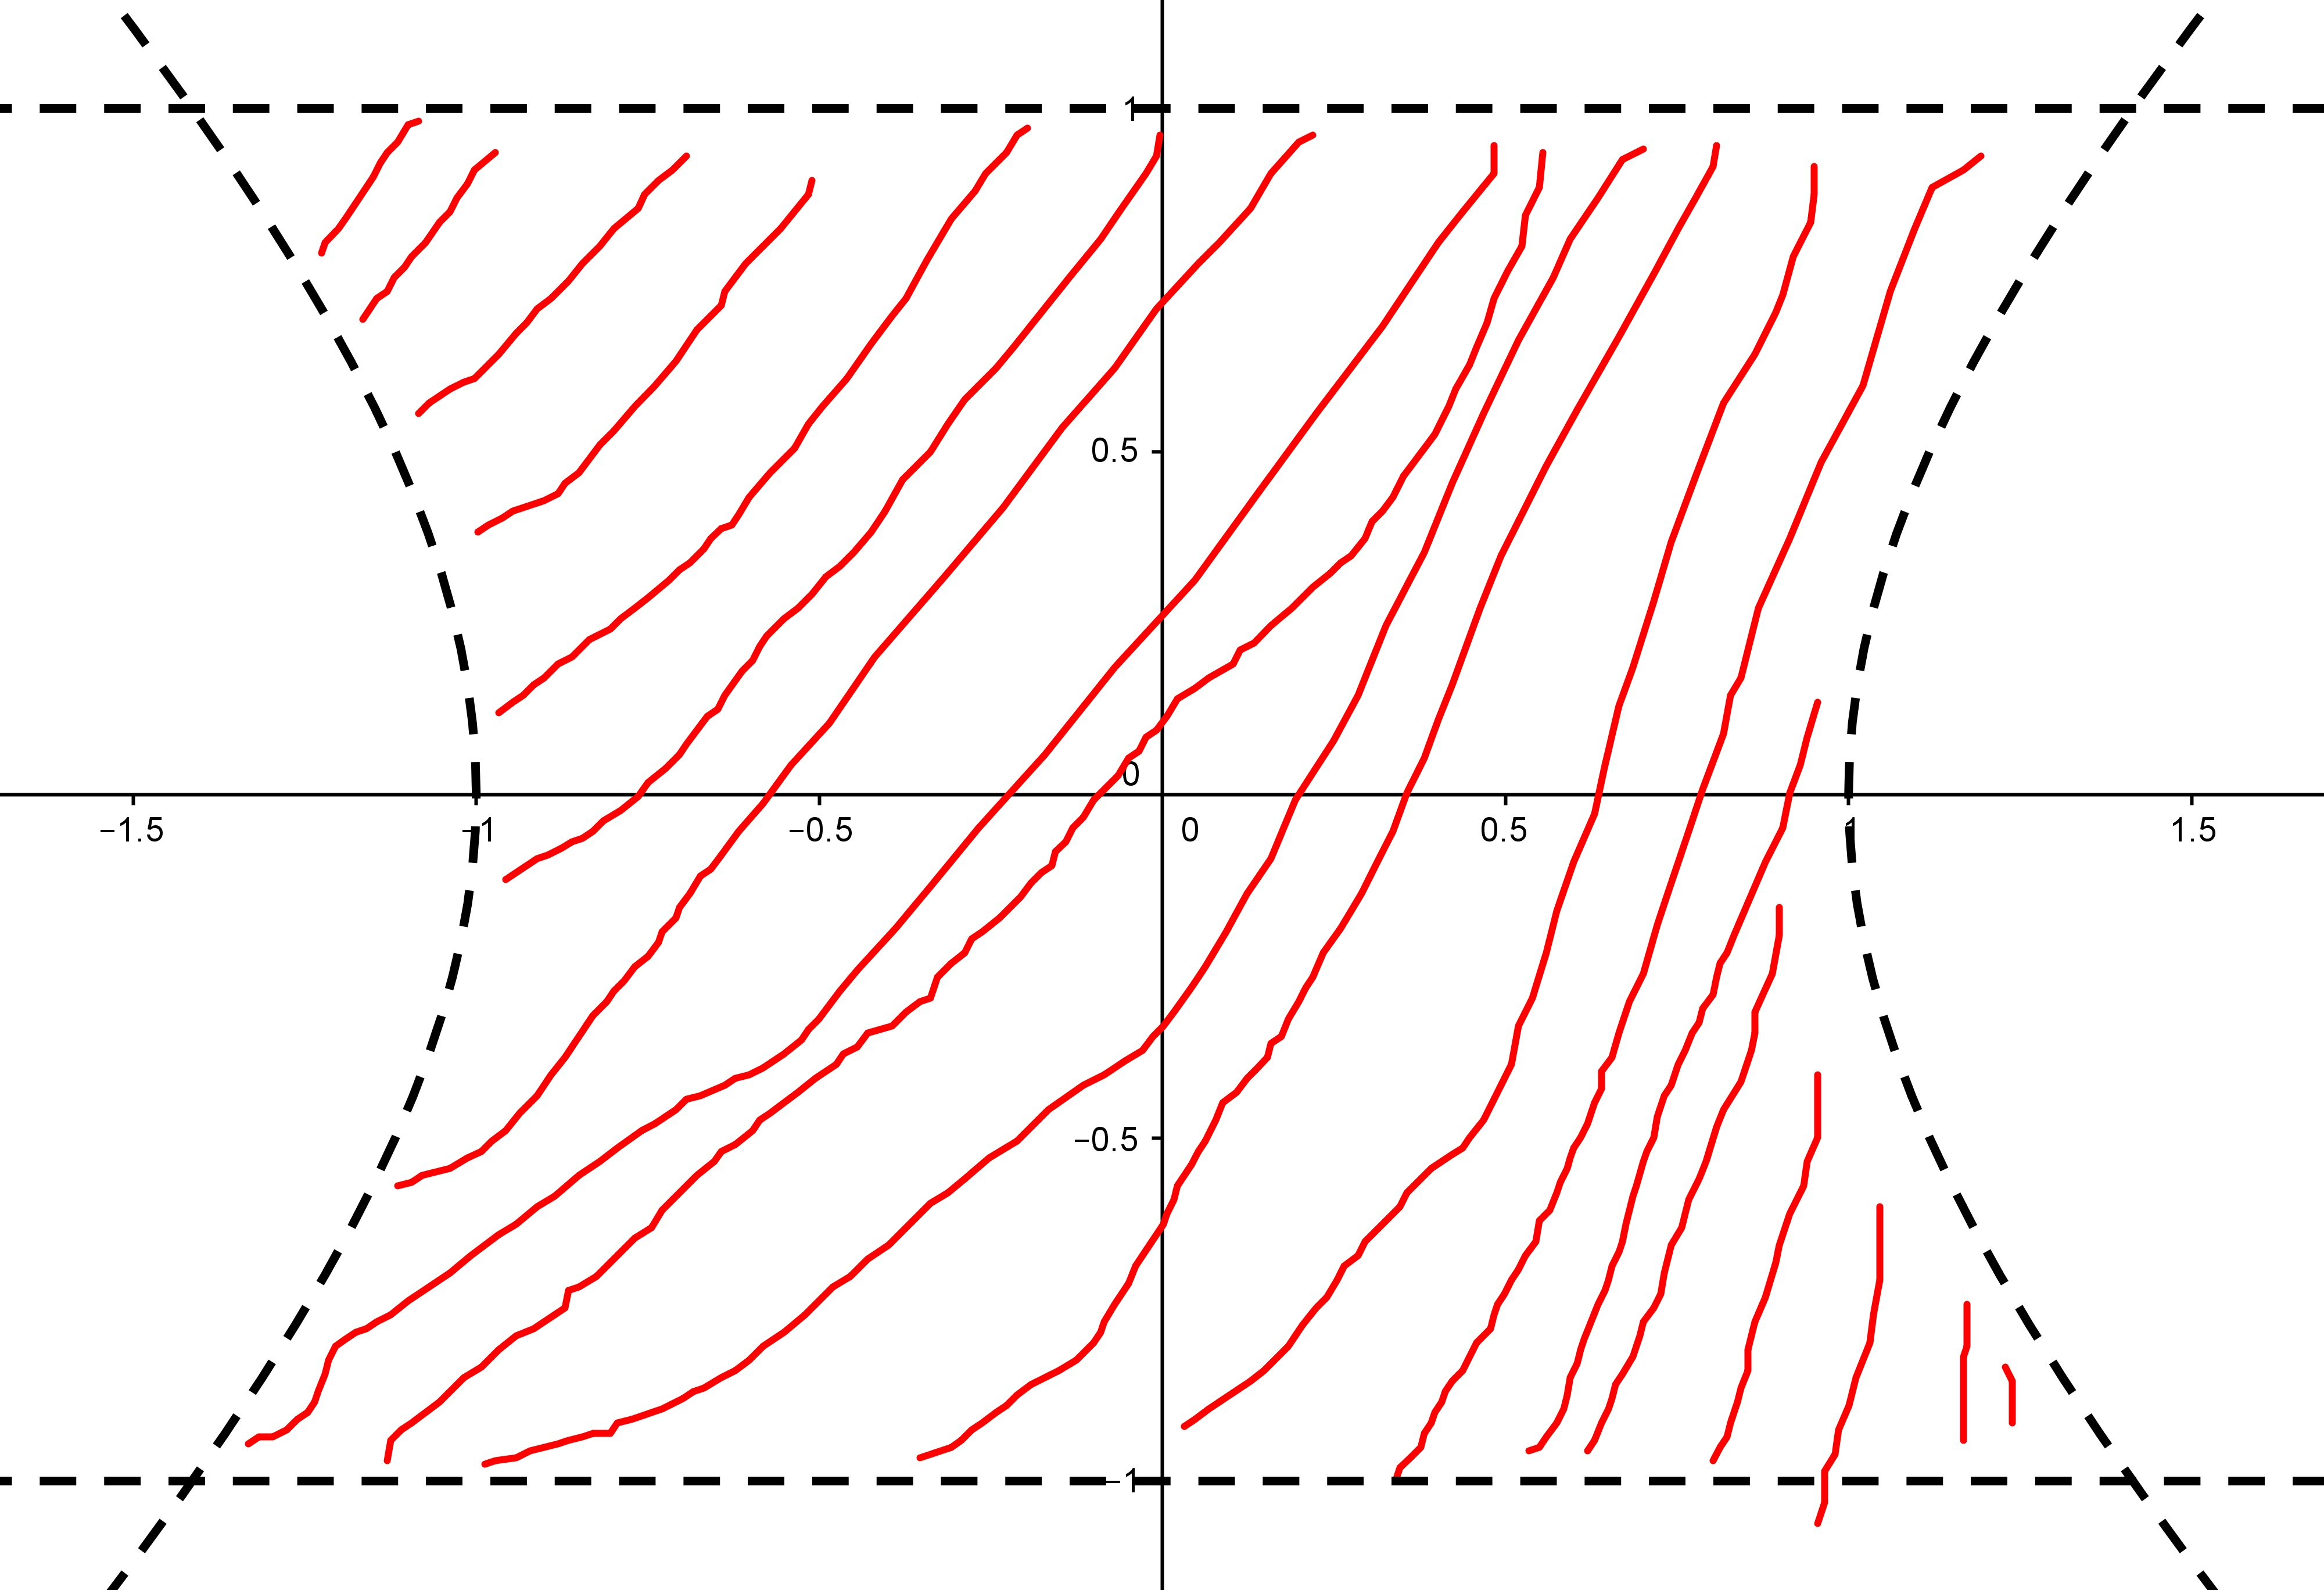
\includegraphics[width=0.7\textwidth]{fig_8_4_2_d}
\captionof{figure}{}
\label{fig:8.4.2_d}
\end{minipage}

$E^\circ = E = \{(x,y):x^2-y^2<1,-1<y<1\}$.

$\overline{\rm E} =  \{(x,y):x^2-y^2\leq 1,-1\leq y\leq 1\}$.

$\partial E = \{(x,y):x^2-y^2 = 1,-1\leq y\leq 1\} \cup \{(x,1):-\sqrt{2}\leq x \leq \sqrt{2}\} \cup \{(x,-1):-\sqrt{2}\leq x \leq \sqrt{2}\}$.
\end{sketch}

\end{enumerate}
\end{Exercise}